\documentclass[article,letterpaper,11pt,oldfontcommands]{memoir}

\setlrmarginsandblock{1.0in}{1.0in}{*}
\setulmarginsandblock{0.5in}{1.0in}{*}
\checkandfixthelayout%

\usepackage{graphicx}      % graphics
\usepackage{amsmath}       % AMS math env
\usepackage{amssymb}       % AMS symbols
\usepackage{caption}       % for subfigures
\usepackage{subcaption}    % |-> this too
\usepackage{array}         % better array environments
\usepackage{booktabs}      % nicer tables/array
\usepackage{tabularx}      % for tabular spacing
\usepackage{mathtools}     % for things like coloneqq
\usepackage{enumerate}     % better enumerate environments
\usepackage{bm} % Bold symbols

\usepackage[default,light]{sourcesanspro}

\usepackage{color}
\definecolor{myred}{RGB}{155,77,40}
\definecolor{UIblue}{RGB}{19,41,75}

\def\Vhrulefill{\leavevmode\leaders\hrule height 0.75ex depth \dimexpr0.4pt-0.7ex\hfill\kern0pt}
\usepackage[explicit]{titlesec}
\titleformat{\section}[runin]{\Large\bfseries\color{UIblue}}{\thesection.}{2.0em}{#1~\Vhrulefill\bigskip\newline}
\titleformat{\subsection}[runin]{\normalsize\bfseries\color{UIblue}}{\thesubsection.}{1.0em}{}
\titlespacing{\section}{0pt}{5pt}{1pt}
\titlespacing{\subsection}{0pt}{-1pt}{1pt}
\renewcommand{\bibname}{\Large\bfseries\color{UIblue}References~\Vhrulefill}

\usepackage{titling}
\setlength{\parskip}{1.5\baselineskip}

\usepackage{tikz}

\pretitle{\begin{flushleft}\LARGE\bfseries}
\posttitle{\par\end{flushleft}}
\preauthor{\begin{flushleft}\large}
\postauthor{\par\end{flushleft}}

\title{\usefont{T1}{qhv}{b}{n}\selectfont Multigrid Methods~---~An Overview}
\author{Luke Olson\\University of Illinois at Urbana-Champaign\\Nelder Felow~--~Imperial College\\
\medskip
\textbf{W May 06 2020, 4--6pm BST}\\
\textbf{F May 08 2020, 4--6pm BST}\\
\textbf{M May 11 2020, 4--6pm BST}\\
\textbf{F May 15 2020, 4--6pm BST}
}
\date{}

\begin{document}
\maketitle

\begin{tikzpicture}[overlay,remember picture]
 \node[anchor=north west,inner sep=0pt] at
   ([xshift=12cm,yshift=-5.8cm]current page.north west)
   {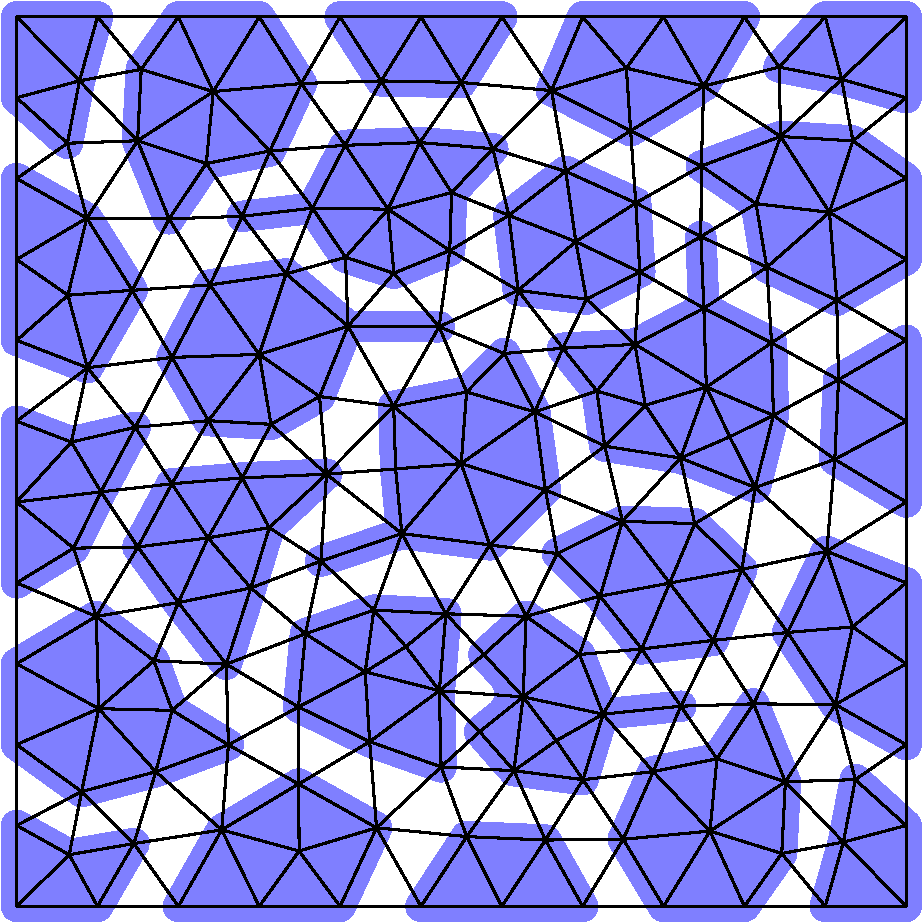
\includegraphics[height=3cm]{graph-aggregates.pdf}};
 \node[anchor=north west,inner sep=0pt] at
   ([xshift=16cm,yshift=-5.8cm]current page.north west)
   {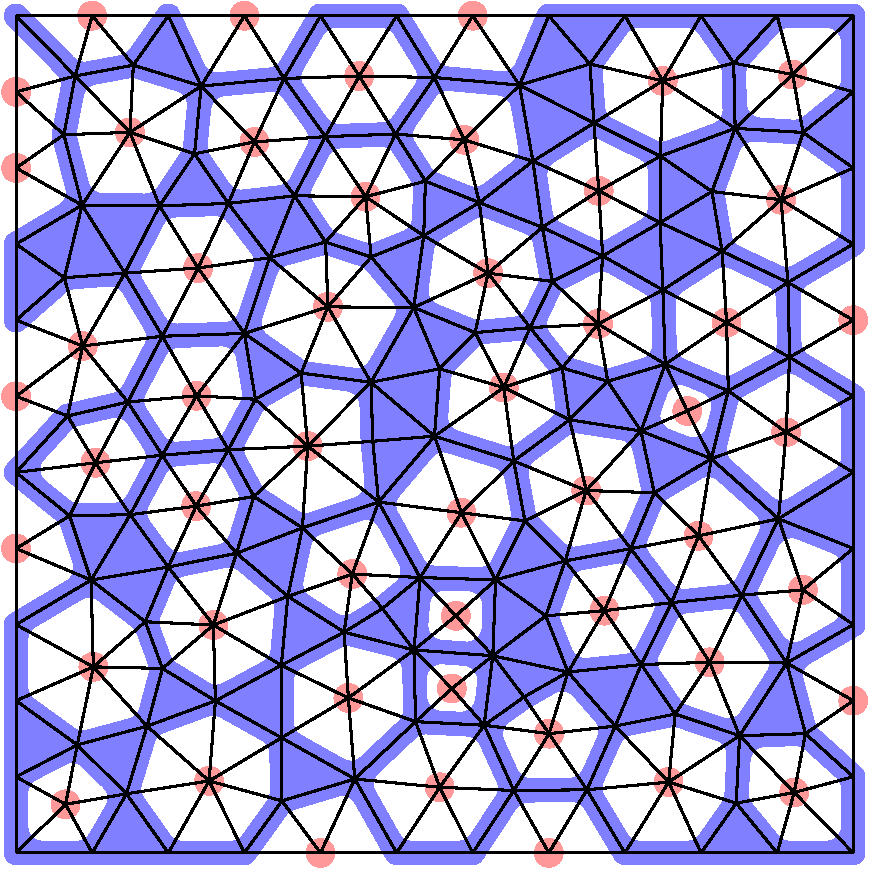
\includegraphics[height=3cm]{graph-splitting.pdf}};
   %\includegraphics[height=3cm]{resimg01.png}
   %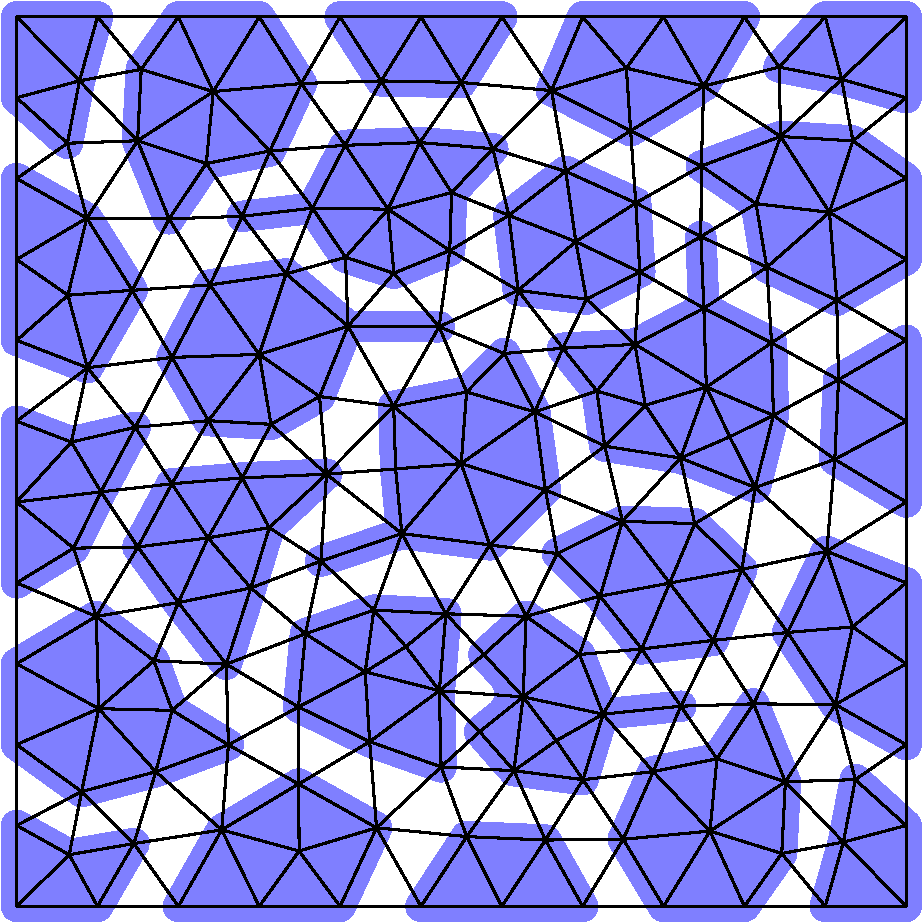
\includegraphics[height=3cm]{graph-aggregates.pdf}
   %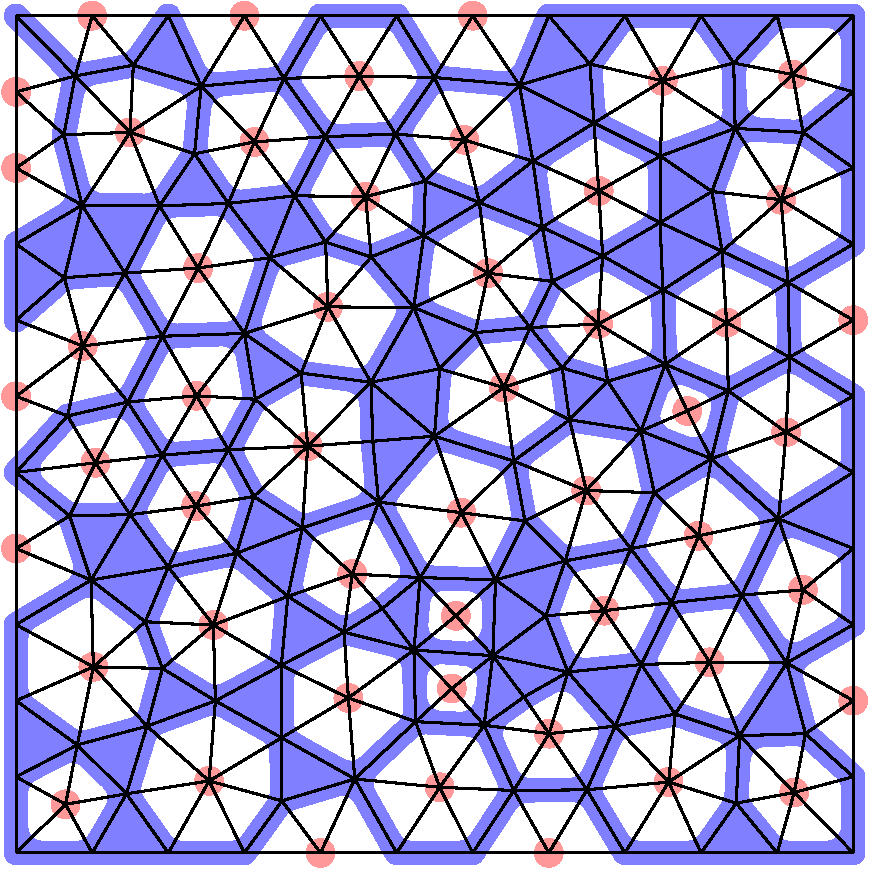
\includegraphics[height=3cm]{graph-splitting.pdf}
   %\includegraphics[height=3cm]{resimg03.png}
\end{tikzpicture}
\vspace{-1.5in}

%done
%    Short CV of the applicant (max 2 pages),
%    List of publications.
%
%    Case for support, including outline and motivation of lecture series or
%    mini-course (max 2 pages),
%
%    Budget, including explicit motivated expression of the requested
%    Fellowship support (with £5,000 max). Where relevant, complementary
%    sources of support should be declared (max 1 page),
%
%    Referees (max 4).
%    Gropp, Manteuffel, McCormick, Heath

\section*{Goals}

The focus of this lecture series is on the fundamentals of multigrid methods
and is open to both practitioners and methods developers in mathematics, computer
science, and the applied sciences. The lecture series will cover the basics of
multigrid methods in both a geometric and algebraic setting, introduce some key
concepts in the theoretical treatment of these methods, and highlight their use
in a parallel setting.

\medskip
\textit{Suggested prerequisites: strong background in
  linear algebraic and some exposure to linear solvers; basic Python experience
  (for examples, but not required); general numerical analysis; introductory knowledge of partial
differential equations}.

\section*{Motivation}
The solution of sparse linear systems is a significant computational challenge
in many simulations.  Often these arise from the discretization of partial
differential equations, although the emergence of complex analytics in data
science application has renewed interest in robust solvers.  The focus of this
lecture series is on so-called multigrid solvers, both theory and
practice.

Multigrid methods have a rich history and continue to play a major role as
the primary solver for many applications.  From its inception in the 70s and
through much of the 80s, the focus of much of the multigrid development was on
\textit{geometric} multigrid, a form that relies on inherent structure in the
problem.  The basic framework of an \textit{algebraic} approach took form in
the late 80s and through the 90s, culminating in range of new methods in the
early 2000s for challenging (mostly elliptic) problems.  In recent years we
have observed significant advances in both theory and in application to a vast
number of problems, including non-symmetric problems, systems of partial
differential equations, graph problems, etc.  To this end, one objective of
this lecture series is to provide a survey of the multigrid methodology as well
as modern `best practices'.

\newpage
\section*{Outline}

A goal of the proposed lecture series is to build a working knowledge of
multigrid methods, both geometric and algebraic.  In addition, an objective is
to bring practitioners, both applications researchers and theorticians, up to
speed with the state of the art in the field.  As such, we will cover the basics
of projection methods and geometric-based multigrid, the basics of the
algebraic form of multigrid, best practices in developing principled solvers
for a range of problems, theoretical aspects of algebraic multigrid, and the
implications of these approaches in a parallel setting.

\vspace{-0.5cm}

\begin{description}
  \item[Lecture \#1: The Basics of Multigrid]
    This lecture will cover the basic principles of geometric multigrid, from
    relaxation methods with a \textit{smoothing} property to the introduction
    of a two-level method.  Convergence properties will be outlined and extensions
    to multiple dimensions will be covered.

  \item[Lecture \#2: Toward Algebraic Multigrid]
    This lecture will begin with an overview of limitations of basic geometric multigrid.
    Operator based methods, such as BoxMG will be introduced, and application to nonlinear
    problems will be explored.  The concept of \textit{algebraically smooth} will also be
    used to motivate upcoming lectures.

  \item[Lecture \#3: CF and Smoothed Aggregation Algebraic Multigrid]
    An overview of the two basic forms of algebraic multigrid will be given.
    Classical, splitting-based methods along with aggregation-based approaches
    will be highlighted in detail, with several examples given in context.

  \item[Lecture \#4: Theoretical Aspects of Algebraic Multigrid]
    Multigrid convergence relies on both effective smoothing and robust coarse-grid correction.
    In this lecture, we give an overview of the underlying theory that supports algebraic multigrid
    and highlight several areas in which the theory is expanding.
\end{description}

\end{document}
